\documentclass[11pt]{article}
\usepackage{amsmath}
\usepackage{amsfonts}
\usepackage{amsthm}
\usepackage{graphicx}
\usepackage{amssymb}
\usepackage{slashed}
\usepackage{listings}
\usepackage{color}

%----------------------------------------------------------------------------------------------------------------------------------------
% Defines various parameters for lstlisting for code snippets
\definecolor{dkgreen}{rgb}{0,0.6,0}
\definecolor{gray}{rgb}{0.5,0.5,0.5}
\definecolor{mauve}{rgb}{0.58,0,0.82}
\definecolor{highlight}{RGB}{255,251,204}

\lstset{frame=tb,
  language=R,
  backgroundcolor=\color{highlight},
  aboveskip=3mm,
  belowskip=3mm,
  showstringspaces=false,
  columns=flexible,
  basicstyle={\small\ttfamily},
  numbers=none,
  numberstyle=\tiny\color{gray},
  keywordstyle=\color{blue},
  commentstyle=\color{dkgreen},
  stringstyle=\color{mauve},
  breaklines=true,
  breakatwhitespace=true,
  tabsize=3}
%----------------------------------------------------------------------------------------------------------------------------------------

%----------------------------------------------------------------------------------------------------------------------------------------
% Set page geometry parameters
\textwidth = 6.5 in
\textheight = 8.5 in
\oddsidemargin = 0.0 in
\evensidemargin = 0.0 in
\topmargin = 0.0 in
\headheight = 0.0 in
\headsep = 0.5 in
\parskip = 0.2in
\parindent = 0.0in
%----------------------------------------------------------------------------------------------------------------------------------------

%----------------------------------------------------------------------------------------------------------------------------------------
%Defines macros for some mathematical tools.  Probably not useful here.
\providecommand{\abs}[1]{\lvert#1\rvert}
\providecommand{\norm}[1]{\lvert\lvert#1\rvert\lvert}
\providecommand{\inner}[2]{\langle#1 , #2\rangle}
\providecommand{\unionover}[3]{ {\underset{#1 \in #2}{\bigcup}} {#3}}
\providecommand{\intover}[3]{ {\underset{#1 \in #2}{\bigcap}} {#3}}

\providecommand{\code}[1]{{\color{red}\ttfamily #1}}
%----------------------------------------------------------------------------------------------------------------------------------------
\begin{document}
\section*{Chapter 5}
\begin{enumerate}
%----------------------------------------------------------------------------------------------------------------------------------------
%----------------------------------------------------------------------------------------------------------------------------------------
\subsection*{Conceptual}

\item Using basic statistical properties of the variance, as well as single variable calculus, derive
\begin{equation}
\alpha=\frac{\sigma_Y^2-\sigma_{XY}}{\sigma_X^2+\sigma_Y^2-2\sigma_{XY}}.
\end{equation}
In other words, prove that $\alpha$ given by the above formula does indeed minimize $\text{Var}(\alpha X+(1-\alpha)Y)$.
\begin{proof}
Let $X$ and $Y$ be random variables and define $f(\alpha)=\text{Var}(\alpha X+(1-\alpha)Y)$.  We first note that $\text{Var}(\alpha X+(1-\alpha)Y)=\alpha^2\text{Var}(X)+(1-\alpha)^2\text{Var}(Y)+2\alpha(1-\alpha)\text{Cov}(X,Y)=\alpha^2(\sigma^2_X+\sigma^2_Y-2\sigma_{XY})-2\alpha(\sigma^2_Y-\sigma_{XY})+\sigma^2_Y$ for each $\alpha\in\mathbb{R}$.  Thus $f$ is quadratic in $\alpha$ with positive leading coefficient and hence has a minimum which must occur at its unique critical point.  Now $\frac{d}{d\alpha} f = 2\alpha(\sigma^2_X+\sigma^2_Y-2\sigma_{XY})-2(\sigma^2_Y-\sigma_{XY})$ and hence $f$ is critical at $\alpha=\frac{\sigma^2_Y-\sigma_{XY}}{\sigma^2_X+\sigma^2_Y-2\sigma_{XY}}$.  Therefore , $f$ has a (unique) minimum at $\alpha=\frac{\sigma^2_Y-\sigma_{XY}}{\sigma^2_X+\sigma^2_Y-2\sigma_{XY}}$.
\end{proof}

\item We will now derive the probability that a given observation is part of a bootstrap sample.  Suppose that we obtain a bootstrap sample from a set of $n$ observations.
\begin{enumerate}
\item What is the probability that the first bootstrap observation is not the $j$th observation from the original sample?  Justify your answer.

Since the first bootstrap observation is chosen uniformly from a population of $n$ objects, the probability that the first observation is any given observation is $\frac{1}{n}$.  Thus the probability that the first observation is not the $j$th element is $1-\frac{1}{n}$.\\

\item What is the probability that the second bootstrap observation is not the $j$th observation from the original sample?

The probability is again $1-\frac{1}{n}$ for the same reasons as above.\\

\item Argue that the probability that the $j$th observation is not in the bootstrap sample is $(1-\frac{1}{n})^n$.

Since each observation has a probability of $1-\frac{1}{n}$ of not picking the $j$th element and the $n$ bootstrap observations are made independently and with replacement the probability that the bootstrap sample does not contain the $j$ observation is $(1-\frac{1}{n})^n$.\\

\item When $n=5$, what is the probability that the $j$th observation is in the bootstrap sample?

$P(j\in B)=1-(1-\frac{1}{5})^5\approx 0.672$\\

\item When $n=100$, what is the probability that the $j$th observation is in the bootstrap sample?

$P(j\in B)=(1-\frac{1}{100})^{100}\approx 0.634$\\

\item When $n=10,000$, what is the probability that the $j$th observation is in the bootstrap sample?

$P(j\in B)=(1-\frac{1}{10000})^{10000}\approx 0.632$\\

\item Create a plot that displays, for each integer value of $n$ from 1 to 100,000, the probability that the $j$th observation is in the bootstrap sample.  Comment on what you observe.

\begin{lstlisting}
> p=function(n){return(1-(1-1/n)^n)}
> plot(x=1:100,p(x))
\end{lstlisting}

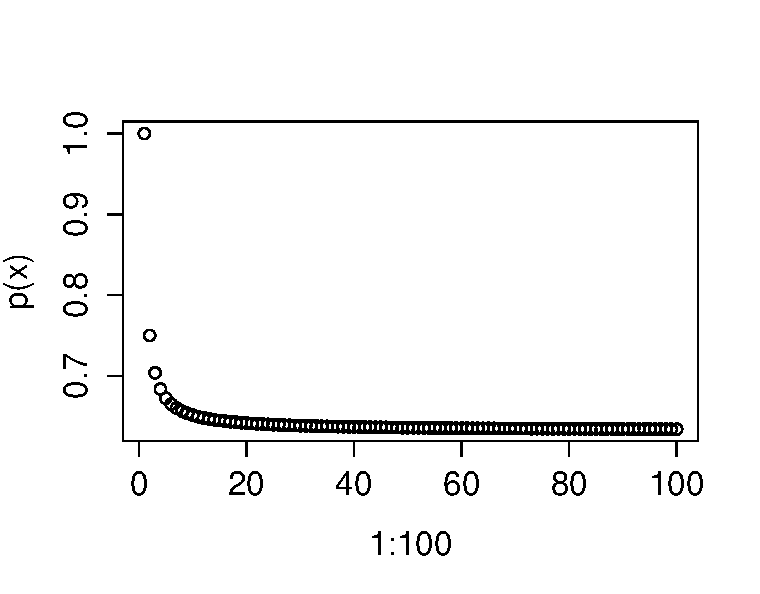
\includegraphics[scale=1]{plot1}

The graph rapidly decreases to an asymptote $p(x)=\frac{e-1}{e}$.\\

\item We will now investigate numerically the probability that a bootstrap sample of size $n=100$ contains the $j$th observation.  Here $j=4$.  We repeatedly create bootstrap samples, and each time we record whether or not the fourth observation is contained in the bootstrap sample.
\begin{lstlisting}
> store=rep(NA,10000)
> for(i in 1:10000){
	store[i]=sum(sample(1:100), rep=TRUE)==4)>0
   }
> mean(store)   
\end{lstlisting}
Comment on the results obtained.

\begin{lstlisting}
[1] 0.6467
\end{lstlisting}

These results are in line with the exact result in (e).
\end{enumerate}

\item We now review $k$-fold cross-validation.
\begin{enumerate}
\item Explain how $k$-fold cross-validation is implemented.

$k$-fold cross-validation is implemented by first partitioning the sample into $k$ subset.  Then for each of the $k$ subsets the desired model is fit to the union of the remaining $k-1$ subsets.  An error statistic (MSE in the case of regression and error rate in the case of classification) is then computed using the held out subset.  Finally, the overall error statistic and its standard error are estimated using the mean and standard deviation, resp.,  of the $k$ subset error statistics.\\

\item What are the advantages and disadvantages of $k$-fold cross-validation relative to:
\begin{enumerate}
\item The validation set approach?

$k$-fold cross-validation is more computationally expensive than the validation set approach.  It is however more accurate, since the error statistic is estimated using multiple fit models each of which utilizes more of the training data.  In particular, $k$-fold cross-validation will have much lower bias.\\
\item LOOCV?

$k$-fold cross-validation is less computationally expensive than LOOCV since it fits fewer models to the data (assuming $k<n$).  LOOCV has the benefit of producing a deterministic estimate of the error statistic, whereas the $k$-fold cross-validation estimate will depend on the choice of partition.  LOOCV will have lower bias, but a higher variance.
\end{enumerate}
\end{enumerate}

\item Suppose that we use some statistical learning method to make a prediction for the response $Y$ for a particular value of the predictor $X$.  Carefully describe how we might estimate the standard deviation of our prediction. 

We can use the bootstrap to estimate the standard deviation of our prediction.  From our training data we repeatedly generate new training sets by sampling from the original training set with replacement.  For each of these bootstrap samples we fit our desired learning method to generate a prediction for $Y$ for the given $X$.  We can then estimate the standard error in our prediction by using the standard deviation of the collection of resampled predictions.

\subsection*{Applied}
\item In Chapter 4, we used logistic regression to predict the probability of \code{default} using \code{income} and \code{balance} on the \code{Default} data set.  We will now estimate the test error of this logistic regression model using the validation set approach.  Do not forget to set a random seed before beginning your analysis.
\begin{enumerate}
\item Fit a logistic regression model that uses \code{income} and \code{balance} to predict \code{default}.
\begin{lstlisting}
> library(ISLR)
> attach(Default)
> set.seed(1)
> glm.fit=glm(default~income+balance, data=Default, family=binomial)
> summary(glm.fit)

Call:
glm(formula = default ~ income + balance, family = binomial, 
    data = Default)

Deviance Residuals: 
    Min       1Q   Median       3Q      Max  
-2.4725  -0.1444  -0.0574  -0.0211   3.7245  

Coefficients:
              Estimate Std. Error z value Pr(>|z|)    
(Intercept) -1.154e+01  4.348e-01 -26.545  < 2e-16 ***
income       2.081e-05  4.985e-06   4.174 2.99e-05 ***
balance      5.647e-03  2.274e-04  24.836  < 2e-16 ***
---
Signif. codes:  0 �***� 0.001 �**� 0.01 �*� 0.05 �.� 0.1 � � 1

(Dispersion parameter for binomial family taken to be 1)

    Null deviance: 2920.6  on 9999  degrees of freedom
Residual deviance: 1579.0  on 9997  degrees of freedom
AIC: 1585

Number of Fisher Scoring iterations: 8
\end{lstlisting}

\item Using the validation set approach, estimate the test error of this model.  In order to do this, you must perform the following steps:
\begin{enumerate}
\item Split the sample set into a training set and a validation set.
\item Fit a multiple logistic regression model using only the training observations.
\item Obtain a prediction of default status for each individual in the validation set by computing the posterior probability of default for that individual, and classifying the individual to the \code{default} category if the posterior probability is greater than $0.5$.
\item Compute the validation set error, which is the fraction of the observations in the validation set that are misclassified.
\end{enumerate}
\begin{lstlisting}
> estimateError=function(){
+     train=sample(length(default),length(default)/2)
+     glm.fit=glm(default~income+balance, data=Default, family=binomial, subset=train)
+     fit.probs=predict(glm.fit, Default[-train,], type="response")
+     fit.pred=rep("No", length(default)/2)
+     fit.pred[fit.probs>0.5]="Yes"
+     return(mean(fit.pred!=Default[-train,][1]))
+ }
> estimateError()
[1] 0.0286
\end{lstlisting}

\item Repeat the process in (b) three times, using three different splits of the observations into training and validation sets.  Comment on the results obtained.
\begin{lstlisting}
> estimateError()
[1] 0.0236
> estimateError()
[1] 0.028
> estimateError()
[1] 0.0268
\end{lstlisting}

The estimates are comparable and vary by less than $0.1\%$.\\
\item Now consider a logistic regression model that predicts the probability of \code{default} using \code{income}, \code{balance} and a dummy variable for \code{student}.  Estimate the test error for this model using the validation set approach.  Comment on whether or not including a dummy variable for \code{student} leads to a reduction in the test error rate.
\begin{lstlisting}
> estimateError=function(){
+     train=sample(length(default),length(default)/2)
+     glm.fit=glm(default~income+balance+student, data=Default, family=binomial, subset=train)
+     fit.probs=predict(glm.fit, Default[-train,], type="response")
+     fit.pred=rep("No", length(default)/2)
+     fit.pred[fit.probs>0.5]="Yes"
+     return(mean(fit.pred!=Default[-train,][1]))
+ }
> estimateError()
[1] 0.0264
\end{lstlisting}

The inclusion of student in the model does not seem to reduce test error.
\end{enumerate}

\item We continue to consider the use of a logistic regression model to predict the probability of \code{default} using \code{income} and \code{balance} on the \code{Default} data set.  In particular, we will now compute estimates for the standard errors of the \code{income} and \code{balance} logistic regression coefficients in two different ways: (1) using the bootstrap, and (2) using the standard formula for computing the standard errors in the \code{glm()} function.
\begin{enumerate}
\item Using the \code{summary()} and \code{glm()} functions, determine the estimated standard errors for the coefficients associated with \code{income} and \code{balance} in the multiple logistic regression model that uses both predictors.

\begin{lstlisting}
> library(ISLR)
> attach(Default)
> set.seed(1)
> glm.fit=glm(default~income+balance, data=Default, family=binomial)
> summary(glm.fit)

Call:
glm(formula = default ~ income + balance, family = binomial, 
    data = Default)

Deviance Residuals: 
    Min       1Q   Median       3Q      Max  
-2.4725  -0.1444  -0.0574  -0.0211   3.7245  

Coefficients:
              Estimate Std. Error z value Pr(>|z|)    
(Intercept) -1.154e+01  4.348e-01 -26.545  < 2e-16 ***
income       2.081e-05  4.985e-06   4.174 2.99e-05 ***
balance      5.647e-03  2.274e-04  24.836  < 2e-16 ***
---
Signif. codes:  0 �***� 0.001 �**� 0.01 �*� 0.05 �.� 0.1 � � 1

(Dispersion parameter for binomial family taken to be 1)

    Null deviance: 2920.6  on 9999  degrees of freedom
Residual deviance: 1579.0  on 9997  degrees of freedom
AIC: 1585

Number of Fisher Scoring iterations: 8
\end{lstlisting}

\item Write a function \code{boot.fn()}, that takes as input the \code{Default} data set as well as an index of the observations, and that outputs the coefficient estimates for \code{income} and \code{balance} in the multiple regression model.
\begin{lstlisting}
> boot.fn=function(data,index){
+     glm.fit=glm(default~income+balance, data=data, family=binomial, subset=index)
+     return(glm.fit$coefficients[2:3])
+ }
> boot.fn(Default, rep(TRUE,length(balance)))
      income      balance 
2.080898e-05 5.647103e-03 
\end{lstlisting}

\item Use the \code{boot()} function together with your \code{boot.fn()} function to estimate the standard errors of the logistic regression coefficients for \code{income} and \code{balance}.
\begin{lstlisting}
> library(boot)
> boot(Default,boot.fn,50)

ORDINARY NONPARAMETRIC BOOTSTRAP


Call:
boot(data = Default, statistic = boot.fn, R = 50)


Bootstrap Statistics :
        original        bias     std. error
t1* 2.080898e-05  2.336088e-07 4.861065e-06
t2* 5.647103e-03 -3.906737e-05 2.392097e-04
\end{lstlisting}

\item Comment on the estimated standard errors obtained using the \code{glm()} function and using your bootstrap function.

The standard errors obtained from the bootstrap are roughly similar to those obtained from glm().
\end{enumerate}

\item In Sections 5.3.2 and 5.3.3, we saw that the \code{cv.glm()} function can be used in order to compute the LOOCV test error estimate.  Alternatively, one could compute those quantities using just the \code{glm()} and \code{predict.glm()} functions, and a for loop.  You will now take this approach in order to compute the LOOCV error for a simple logistic regression model on the \code{Weekly} data set.  Recall that in the context of classification problems, the LOOCV error is given by
\begin{equation}
CV_n=\frac{1}{n}\sum_{i=1}^n Err_i
\end{equation}
\begin{enumerate}
\item Fit a logistic regression model that predicts \code{Direction} using \code{Lag1} and \code{Lag2}.
\begin{lstlisting}
> attach(Weekly)
> glm.fit=glm(Direction~Lag1+Lag2, data=Weekly, family=binomial)
> summary(glm.fit)

Call:
glm(formula = Direction ~ Lag1 + Lag2, family = binomial, data = Weekly)

Deviance Residuals: 
   Min      1Q  Median      3Q     Max  
-1.623  -1.261   1.001   1.083   1.506  

Coefficients:
            Estimate Std. Error z value Pr(>|z|)    
(Intercept)  0.22122    0.06147   3.599 0.000319 ***
Lag1        -0.03872    0.02622  -1.477 0.139672    
Lag2         0.06025    0.02655   2.270 0.023232 *  
---
Signif. codes:  0 �***� 0.001 �**� 0.01 �*� 0.05 �.� 0.1 � � 1

(Dispersion parameter for binomial family taken to be 1)

    Null deviance: 1496.2  on 1088  degrees of freedom
Residual deviance: 1488.2  on 1086  degrees of freedom
AIC: 1494.2

Number of Fisher Scoring iterations: 4
\end{lstlisting}

\item Fit a logistic regression model that predicts \code{Direction} using \code{Lag1} and \code{Lag2} using all but the first observation.
\begin{lstlisting}
> glm.fit=glm(Direction~Lag1+Lag2, data=Weekly[-1,], family=binomial)
> summary(glm.fit)

Call:
glm(formula = Direction ~ Lag1 + Lag2, family = binomial, data = Weekly[-1, 
    ])

Deviance Residuals: 
    Min       1Q   Median       3Q      Max  
-1.6258  -1.2617   0.9999   1.0819   1.5071  

Coefficients:
            Estimate Std. Error z value Pr(>|z|)    
(Intercept)  0.22324    0.06150   3.630 0.000283 ***
Lag1        -0.03843    0.02622  -1.466 0.142683    
Lag2         0.06085    0.02656   2.291 0.021971 *  
---
Signif. codes:  0 �***� 0.001 �**� 0.01 �*� 0.05 �.� 0.1 � � 1

(Dispersion parameter for binomial family taken to be 1)

    Null deviance: 1494.6  on 1087  degrees of freedom
Residual deviance: 1486.5  on 1085  degrees of freedom
AIC: 1492.5

Number of Fisher Scoring iterations: 4
\end{lstlisting}

\item Use the model from (b) to predict the direction of the first observation.  You can do this by predicting that the first observation will go up if $P(\text{Direction=="Up"}|\text{Lag1,Lag2})>0.5$.  Was this observation correctly classified?
\begin{lstlisting}
> predict.glm(glm.fit, Weekly[1,], type="response")>0.5
   1 
TRUE 
> Direction[1]
[1] Down
Levels: Down Up
\end{lstlisting}
The model predicted that the first observation would be an Up.  The true observation is Down.

\item Write a for loop from $i=1$ to $i=n$, where $n$ is the number of observations in the data set, that performs each of the following steps:
\begin{enumerate}
\item Fit a logistic regression model using all but the $i$th observation to predict \code{Direction} using \code{Lag1} and \code{Lag2}.
\item Compute the posterior probability of the market moving up for the $i$th observation.
\item Use the posterior probability for the $i$th observation in order to predict whether or not the market moves up.
\item Determine whether or not an error was made in predicting the direction for the $i$th observation.  If an error was made indicate this as a 1, and otherwise indicate it as a 0. 
\end{enumerate}
\begin{lstlisting}
> for (i in 1:length(Direction)){
+     glm.fit=glm(Direction~Lag1+Lag2, data=Weekly[-i,], family=binomial)
+     pred_up=predict.glm(glm.fit, Weekly[i,], type="response")>0.5
+     if ((pred_up && Direction[i]!="Up")||(!pred_up && Direction[i]=="Up"))
+          results[i]=1
+ }
\end{lstlisting}

\item Take the average of the $n$ numbers obtained in (d) in order to obtain the LOOCV estimate for the test error.  Comment on the results.
\begin{lstlisting}
> mean(results)
[1] 0.4499541
\end{lstlisting}

LOOCV estimates the test error rate of the model is $45\%$.
\end{enumerate}

\item We will now perform cross-validation on a simulated data set.
\begin{enumerate}
\item Generate a simulated data set as follows:
\begin{lstlisting}
> set.seed(1)
> y=rnorm(100)
> x=rnorm(100)
> y=x-2*x^2+rnorm(100)
\end{lstlisting}
In this data set, what is $n$ and what is $p$?  Write out the model used to generate the data in equation form.

In this data set $n=100$ and $p=2$.  The data are generated by
\begin{equation}
Y=X-2X^2+\epsilon,
\end{equation}
where $X,\epsilon \sim N(0,1)$.

\item Create a scatterplot of $X$ against $Y$.  Comment on what you find.

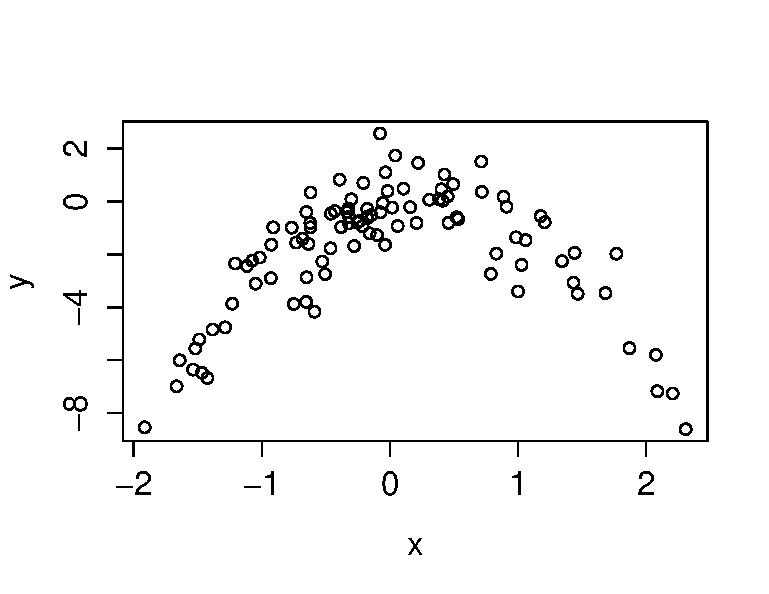
\includegraphics{plot2}

As expected, the data appear quadratic in $x$.

\item Set a random seed, and then compute the LOOCV errors that result from fitting the following four models using least squares:
\begin{enumerate}
\item $Y=\beta_0+\beta_1 X +\epsilon$
\item $Y=\beta_0+\beta_1 X +\beta_2 X^2+\epsilon$
\item $Y=\beta_0+\beta_1 X +\beta_2 X^2+\beta_3 X^3+\epsilon$
\item $Y=\beta_0+\beta_1 X +\beta_2 X^2+\beta_3 X^3+\beta_4 X^4+\epsilon$
\end{enumerate}
Note you may find it helpful to use the \code{data.frame()} function to create a single data set containing both $X$ and $Y$.

\begin{lstlisting}
> library(boot)
> Data=data.frame(x,y)
> set.seed(1)
> glm.fit=glm(y~x)
> cv.glm(Data,glm.fit)$delta
[1] 5.890979 5.888812
\end{lstlisting}

\begin{lstlisting}
> glm.fit=glm(y~poly(x,2))
> cv.glm(Data,glm.fit)$delta
[1] 1.086596 1.086326
\end{lstlisting}

\begin{lstlisting}
> glm.fit=glm(y~poly(x,3))
> cv.glm(Data,glm.fit)$delta
[1] 1.102585 1.102227
\end{lstlisting}

\begin{lstlisting}
> glm.fit=glm(y~poly(x,4))
> cv.glm(Data,glm.fit)$delta
[1] 1.114772 1.114334
\end{lstlisting}

\item Repeat (c) using another random seed, report your results.  Are your results the same as what you got in (c)? Why?

\begin{lstlisting}
> set.seed(27)
> glm.fit=glm(y~x)
> cv.glm(Data,glm.fit)$delta
[1] 5.890979 5.888812
> glm.fit=glm(y~poly(x,2))
> cv.glm(Data,glm.fit)$delta
[1] 1.086596 1.086326
> glm.fit=glm(y~poly(x,3))
> cv.glm(Data,glm.fit)$delta
[1] 1.102585 1.102227
> glm.fit=glm(y~poly(x,4))
> cv.glm(Data,glm.fit)$delta
[1] 1.114772 1.114334
\end{lstlisting}

These results are identical to those obtained above.  This is expected since LOOCV always trains the model on all training sets of a  single fewer training example.\\

\item Which of the models in (c) had the smallest LOOCV error?  Is this what you expected?  Explain your answer.

The quadratic fit has the smallest LOOCV error.  This is expected as the simulated data are actually quadratic.  The cubic and quartic fits do a much better job than the linear fit and are only slightly worse than the quadratic fit.\\

\item Comment on the statistical significance of the coefficient estimates that results from fitting each of the models in (c) using least squares.  Do these results agree with the conclusions drawn based on the cross-validation results?
\begin{lstlisting}
> glm.fit=glm(y~poly(x,4))
> summary(glm.fit)

Call:
glm(formula = y ~ poly(x, 4))

Deviance Residuals: 
    Min       1Q   Median       3Q      Max  
-2.8914  -0.5244   0.0749   0.5932   2.7796  

Coefficients:
            Estimate Std. Error t value Pr(>|t|)    
(Intercept)  -1.8277     0.1041 -17.549   <2e-16 ***
poly(x, 4)1   2.3164     1.0415   2.224   0.0285 *  
poly(x, 4)2 -21.0586     1.0415 -20.220   <2e-16 ***
poly(x, 4)3  -0.3048     1.0415  -0.293   0.7704    
poly(x, 4)4  -0.4926     1.0415  -0.473   0.6373    
---
Signif. codes:  0 �***� 0.001 �**� 0.01 �*� 0.05 �.� 0.1 � � 1

(Dispersion parameter for gaussian family taken to be 1.084654)

    Null deviance: 552.21  on 99  degrees of freedom
Residual deviance: 103.04  on 95  degrees of freedom
AIC: 298.78

Number of Fisher Scoring iterations: 2
\end{lstlisting}

In the full model the degree one and two terms are statistically significant, but the degree 3 and 4 terms are not.  This is consistent with the conclusions drawn above from LOOCV.  Inclusion of a degree 2 term significantly improves the model, but there is no need to include higher order terms.
\end{enumerate}

\item We will now consider the \code{Boston} housing data set, from the \code{MASS} library.
\begin{enumerate}
\item Based on this data set, provide an estimate for the population mean of \code{medv}.  Call this estimate $\hat\mu$.
\begin{lstlisting}
> library(MASS)
> attach(Boston)
> mean(medv)
[1] 22.53281
\end{lstlisting}
We estimate $\mu\approx\hat\mu=22.53$.\\

\item Provide an estimate of the standard error of $\hat\mu$. Interpret this result.
\begin{lstlisting}
> sd(medv)/sqrt(length(medv))
[1] 0.4088611
\end{lstlisting}

We estimate $\sigma_{medv}\approx\hat\sigma_{medv}=0.409$.

\item Now estimate the standard error of $\hat\mu$ using the bootstrap.  How does this compare to your answer from (b)?

\begin{lstlisting}
> set.seed(1)
> boot.fn=function(data,index){return(mean(data[index]))}
> strap=boot(medv, boot.fn, 1000)
> strap

ORDINARY NONPARAMETRIC BOOTSTRAP


Call:
boot(data = medv, statistic = boot.fn, R = 1000)


Bootstrap Statistics :
    original      bias    std. error
t1* 22.53281 0.008517589   0.4119374
\end{lstlisting}
The results are very similar, with a bootstrap estimate of $0.412$ as compared to the value of $0.409$ obtained from the formula.\\

\item Based on your bootstrap estimate from (c), provide a $95\%$ confidence interval for the mean of \code{medv}.  Compare it to the results obtained using \code{t.test(Boston\$medv)}.

\begin{lstlisting}
> t.test(Boston$medv)

	One Sample t-test

data:  Boston$medv
t = 55.1111, df = 505, p-value < 2.2e-16
alternative hypothesis: true mean is not equal to 0
95 percent confidence interval:
 21.72953 23.33608
sample estimates:
mean of x 
 22.53281
 
 > c(strap$t0-2*0.4119374, strap$t0+2*0.4119374)
[1] 21.70893 23.35668
\end{lstlisting}

The bootstrap confidence interval is comparable but slightly wider than that obtained by the t-test.\\

\item Based on this data set, provide an estimate, $\hat\mu_{med}$, for the median value of \code{medv} in the population.
\begin{lstlisting}
> median(medv)
[1] 21.2
\end{lstlisting}

\item We now would like to estimate the standard error of $\hat\mu_{med}$.  Unfortunately, there is no simple formula for computing the standard error of the median.  Instead, estimate the standard error of the median using the bootstrap.  Comment on your findings.
\begin{lstlisting}
> set.seed(1)
> boot.fn=function(data,index){return(median(data[index]))}
> strap=boot(medv, boot.fn, 1000)
> strap

ORDINARY NONPARAMETRIC BOOTSTRAP


Call:
boot(data = medv, statistic = boot.fn, R = 1000)


Bootstrap Statistics :
    original   bias    std. error
t1*     21.2 -0.01615   0.3801002
\end{lstlisting}
We find $\hat\mu_{med}=21.2$ with a standard error of $0.380$.  The standard error is smaller than that of the mean estimate, and small relative to $\hat\mu$.

\item Based on this data set, provide an estimate for the tenth percentile of \code{medv} in the Boston suburbs.  Call this quantity $\hat\mu_{0.1}$. 
\begin{lstlisting}
> quantile(medv,0.1)
  10% 
12.75 
\end{lstlisting}

\item Use the bootstrap to estimate the standard error of $\hat\mu_{0.1}$.  Comment on your findings.
\begin{lstlisting}
> boot.fn=function(data,index){return(quantile(data[index],c(0.1)))}
> strap=boot(medv, boot.fn, 1000)
> strap

ORDINARY NONPARAMETRIC BOOTSTRAP


Call:
boot(data = medv, statistic = boot.fn, R = 1000)


Bootstrap Statistics :
    original  bias    std. error
t1*    12.75 0.00165   0.5112202
\end{lstlisting}

We find $\hat\mu_{0.1}=12.75$ with a standard error of $0.511$.  The standard error is larger than that of the mean and median estimates, but still small relative to $\hat\mu_{0.1}$.
\end{enumerate}


















%----------------------------------------------------------------------------------------------------------------------------------------
\end{enumerate}
\end{document}